% Options for packages loaded elsewhere
\PassOptionsToPackage{unicode}{hyperref}
\PassOptionsToPackage{hyphens}{url}
\PassOptionsToPackage{dvipsnames,svgnames,x11names}{xcolor}
%
\documentclass[
  letterpaper,
  DIV=11,
  numbers=noendperiod]{scrartcl}

\usepackage{amsmath,amssymb}
\usepackage{lmodern}
\usepackage{iftex}
\ifPDFTeX
  \usepackage[T1]{fontenc}
  \usepackage[utf8]{inputenc}
  \usepackage{textcomp} % provide euro and other symbols
\else % if luatex or xetex
  \usepackage{unicode-math}
  \defaultfontfeatures{Scale=MatchLowercase}
  \defaultfontfeatures[\rmfamily]{Ligatures=TeX,Scale=1}
\fi
% Use upquote if available, for straight quotes in verbatim environments
\IfFileExists{upquote.sty}{\usepackage{upquote}}{}
\IfFileExists{microtype.sty}{% use microtype if available
  \usepackage[]{microtype}
  \UseMicrotypeSet[protrusion]{basicmath} % disable protrusion for tt fonts
}{}
\makeatletter
\@ifundefined{KOMAClassName}{% if non-KOMA class
  \IfFileExists{parskip.sty}{%
    \usepackage{parskip}
  }{% else
    \setlength{\parindent}{0pt}
    \setlength{\parskip}{6pt plus 2pt minus 1pt}}
}{% if KOMA class
  \KOMAoptions{parskip=half}}
\makeatother
\usepackage{xcolor}
\setlength{\emergencystretch}{3em} % prevent overfull lines
\setcounter{secnumdepth}{-\maxdimen} % remove section numbering
% Make \paragraph and \subparagraph free-standing
\ifx\paragraph\undefined\else
  \let\oldparagraph\paragraph
  \renewcommand{\paragraph}[1]{\oldparagraph{#1}\mbox{}}
\fi
\ifx\subparagraph\undefined\else
  \let\oldsubparagraph\subparagraph
  \renewcommand{\subparagraph}[1]{\oldsubparagraph{#1}\mbox{}}
\fi

\usepackage{color}
\usepackage{fancyvrb}
\newcommand{\VerbBar}{|}
\newcommand{\VERB}{\Verb[commandchars=\\\{\}]}
\DefineVerbatimEnvironment{Highlighting}{Verbatim}{commandchars=\\\{\}}
% Add ',fontsize=\small' for more characters per line
\usepackage{framed}
\definecolor{shadecolor}{RGB}{241,243,245}
\newenvironment{Shaded}{\begin{snugshade}}{\end{snugshade}}
\newcommand{\AlertTok}[1]{\textcolor[rgb]{0.68,0.00,0.00}{#1}}
\newcommand{\AnnotationTok}[1]{\textcolor[rgb]{0.37,0.37,0.37}{#1}}
\newcommand{\AttributeTok}[1]{\textcolor[rgb]{0.40,0.45,0.13}{#1}}
\newcommand{\BaseNTok}[1]{\textcolor[rgb]{0.68,0.00,0.00}{#1}}
\newcommand{\BuiltInTok}[1]{\textcolor[rgb]{0.00,0.23,0.31}{#1}}
\newcommand{\CharTok}[1]{\textcolor[rgb]{0.13,0.47,0.30}{#1}}
\newcommand{\CommentTok}[1]{\textcolor[rgb]{0.37,0.37,0.37}{#1}}
\newcommand{\CommentVarTok}[1]{\textcolor[rgb]{0.37,0.37,0.37}{\textit{#1}}}
\newcommand{\ConstantTok}[1]{\textcolor[rgb]{0.56,0.35,0.01}{#1}}
\newcommand{\ControlFlowTok}[1]{\textcolor[rgb]{0.00,0.23,0.31}{#1}}
\newcommand{\DataTypeTok}[1]{\textcolor[rgb]{0.68,0.00,0.00}{#1}}
\newcommand{\DecValTok}[1]{\textcolor[rgb]{0.68,0.00,0.00}{#1}}
\newcommand{\DocumentationTok}[1]{\textcolor[rgb]{0.37,0.37,0.37}{\textit{#1}}}
\newcommand{\ErrorTok}[1]{\textcolor[rgb]{0.68,0.00,0.00}{#1}}
\newcommand{\ExtensionTok}[1]{\textcolor[rgb]{0.00,0.23,0.31}{#1}}
\newcommand{\FloatTok}[1]{\textcolor[rgb]{0.68,0.00,0.00}{#1}}
\newcommand{\FunctionTok}[1]{\textcolor[rgb]{0.28,0.35,0.67}{#1}}
\newcommand{\ImportTok}[1]{\textcolor[rgb]{0.00,0.46,0.62}{#1}}
\newcommand{\InformationTok}[1]{\textcolor[rgb]{0.37,0.37,0.37}{#1}}
\newcommand{\KeywordTok}[1]{\textcolor[rgb]{0.00,0.23,0.31}{#1}}
\newcommand{\NormalTok}[1]{\textcolor[rgb]{0.00,0.23,0.31}{#1}}
\newcommand{\OperatorTok}[1]{\textcolor[rgb]{0.37,0.37,0.37}{#1}}
\newcommand{\OtherTok}[1]{\textcolor[rgb]{0.00,0.23,0.31}{#1}}
\newcommand{\PreprocessorTok}[1]{\textcolor[rgb]{0.68,0.00,0.00}{#1}}
\newcommand{\RegionMarkerTok}[1]{\textcolor[rgb]{0.00,0.23,0.31}{#1}}
\newcommand{\SpecialCharTok}[1]{\textcolor[rgb]{0.37,0.37,0.37}{#1}}
\newcommand{\SpecialStringTok}[1]{\textcolor[rgb]{0.13,0.47,0.30}{#1}}
\newcommand{\StringTok}[1]{\textcolor[rgb]{0.13,0.47,0.30}{#1}}
\newcommand{\VariableTok}[1]{\textcolor[rgb]{0.07,0.07,0.07}{#1}}
\newcommand{\VerbatimStringTok}[1]{\textcolor[rgb]{0.13,0.47,0.30}{#1}}
\newcommand{\WarningTok}[1]{\textcolor[rgb]{0.37,0.37,0.37}{\textit{#1}}}

\providecommand{\tightlist}{%
  \setlength{\itemsep}{0pt}\setlength{\parskip}{0pt}}\usepackage{longtable,booktabs,array}
\usepackage{calc} % for calculating minipage widths
% Correct order of tables after \paragraph or \subparagraph
\usepackage{etoolbox}
\makeatletter
\patchcmd\longtable{\par}{\if@noskipsec\mbox{}\fi\par}{}{}
\makeatother
% Allow footnotes in longtable head/foot
\IfFileExists{footnotehyper.sty}{\usepackage{footnotehyper}}{\usepackage{footnote}}
\makesavenoteenv{longtable}
\usepackage{graphicx}
\makeatletter
\def\maxwidth{\ifdim\Gin@nat@width>\linewidth\linewidth\else\Gin@nat@width\fi}
\def\maxheight{\ifdim\Gin@nat@height>\textheight\textheight\else\Gin@nat@height\fi}
\makeatother
% Scale images if necessary, so that they will not overflow the page
% margins by default, and it is still possible to overwrite the defaults
% using explicit options in \includegraphics[width, height, ...]{}
\setkeys{Gin}{width=\maxwidth,height=\maxheight,keepaspectratio}
% Set default figure placement to htbp
\makeatletter
\def\fps@figure{htbp}
\makeatother

\KOMAoption{captions}{tableheading}
\makeatletter
\makeatother
\makeatletter
\makeatother
\makeatletter
\@ifpackageloaded{caption}{}{\usepackage{caption}}
\AtBeginDocument{%
\ifdefined\contentsname
  \renewcommand*\contentsname{Table of contents}
\else
  \newcommand\contentsname{Table of contents}
\fi
\ifdefined\listfigurename
  \renewcommand*\listfigurename{List of Figures}
\else
  \newcommand\listfigurename{List of Figures}
\fi
\ifdefined\listtablename
  \renewcommand*\listtablename{List of Tables}
\else
  \newcommand\listtablename{List of Tables}
\fi
\ifdefined\figurename
  \renewcommand*\figurename{Figure}
\else
  \newcommand\figurename{Figure}
\fi
\ifdefined\tablename
  \renewcommand*\tablename{Table}
\else
  \newcommand\tablename{Table}
\fi
}
\@ifpackageloaded{float}{}{\usepackage{float}}
\floatstyle{ruled}
\@ifundefined{c@chapter}{\newfloat{codelisting}{h}{lop}}{\newfloat{codelisting}{h}{lop}[chapter]}
\floatname{codelisting}{Listing}
\newcommand*\listoflistings{\listof{codelisting}{List of Listings}}
\makeatother
\makeatletter
\@ifpackageloaded{caption}{}{\usepackage{caption}}
\@ifpackageloaded{subcaption}{}{\usepackage{subcaption}}
\makeatother
\makeatletter
\@ifpackageloaded{tcolorbox}{}{\usepackage[many]{tcolorbox}}
\makeatother
\makeatletter
\@ifundefined{shadecolor}{\definecolor{shadecolor}{rgb}{.97, .97, .97}}
\makeatother
\makeatletter
\makeatother
\ifLuaTeX
  \usepackage{selnolig}  % disable illegal ligatures
\fi
\IfFileExists{bookmark.sty}{\usepackage{bookmark}}{\usepackage{hyperref}}
\IfFileExists{xurl.sty}{\usepackage{xurl}}{} % add URL line breaks if available
\urlstyle{same} % disable monospaced font for URLs
\hypersetup{
  pdftitle={CI/CD in the \{pharmaverse\}},
  colorlinks=true,
  linkcolor={blue},
  filecolor={Maroon},
  citecolor={Blue},
  urlcolor={Blue},
  pdfcreator={LaTeX via pandoc}}

\title{CI/CD in the \{pharmaverse\}}
\usepackage{etoolbox}
\makeatletter
\providecommand{\subtitle}[1]{% add subtitle to \maketitle
  \apptocmd{\@title}{\par {\large #1 \par}}{}{}
}
\makeatother
\subtitle{R/Pharma

November 10th, 2022

Ben Straub (GSK) \& Craig Gower-Page (Roche)}
\author{}
\date{}

\begin{document}
\maketitle
\ifdefined\Shaded\renewenvironment{Shaded}{\begin{tcolorbox}[enhanced, interior hidden, borderline west={3pt}{0pt}{shadecolor}, breakable, boxrule=0pt, frame hidden, sharp corners]}{\end{tcolorbox}}\fi

\hypertarget{introduction}{%
\section{Introduction}\label{introduction}}

\hypertarget{what-is-cicd}{%
\subsection{What is CI/CD?}\label{what-is-cicd}}

\begin{itemize}
\tightlist
\item
  Continuous Integration (CI): Frequent merging of several small changes
  into a main branch
\item
  Continuous Delivery (CD): Repeatable deployment process when deciding
  to deploy
\end{itemize}

CI/CD bridges the gaps between development and operation activities and
teams by \textbf{enforcing automation} in building, testing and
deployment of applications. CI/CD services compile the incremental code
changes made by developers, then link and package them into software
deliverables

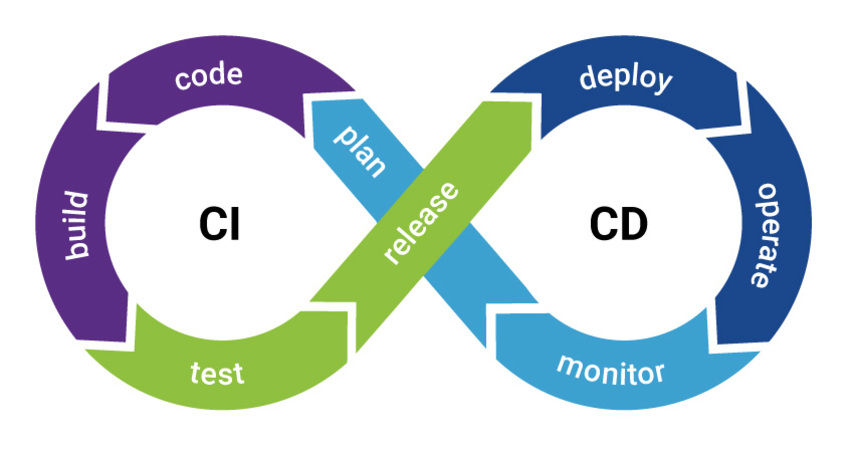
\includegraphics{cicd.jpg}


\includegraphics{pharmaverse.png}

\href{https://en.wikipedia.org/wiki/CI/CD\#cite_note-2}{Wikipedia:
CI/CD} \href{https://github.com/pharmaverse}{\{pharmaverse\}}

\hypertarget{does-it-help}{%
\subsection{Does it help?}\label{does-it-help}}

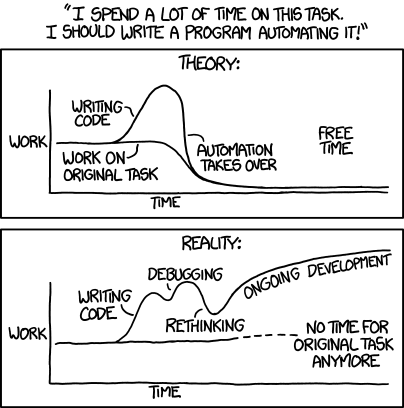
\includegraphics{automation.png}

\begin{itemize}
\tightlist
\item
  \ldots Yes! Yes, it does!!
\end{itemize}

\href{https://xkcd.com/1319/}{XKCD}

\hypertarget{how-does-cicd-help-r-packages}{%
\subsection{How does CI/CD help R
packages?}\label{how-does-cicd-help-r-packages}}

\begin{itemize}
\tightlist
\item
  Catch issues (bugs) early on
\item
  User base on multiple OSes and multiple R versions
\item
  Faster turnaround on Code Review
\item
  Multiple Contributors on your R Package
\item
  Enforce style conventions and preferences
\item
  Measure test coverage for new code
\item
  Keep docs up-to-date
\item
  And we can just keep going!
\end{itemize}

\hypertarget{what-could-standard-cicd-for-r-packages-look-like}{%
\subsection{What could standard CI/CD for R packages look
like?}\label{what-could-standard-cicd-for-r-packages-look-like}}

\begin{itemize}
\tightlist
\item
  Not all R packages are the same, but they are still pretty similar!
\end{itemize}

\begin{enumerate}
\def\labelenumi{\arabic{enumi}.}
\tightlist
\item
  Unit Tests
\item
  Link \& URL Checks
\item
  Spelling Checks
\item
  Static Code Analysis
\end{enumerate}

\begin{enumerate}
\def\labelenumi{\arabic{enumi}.}
\setcounter{enumi}{4}
\tightlist
\item
  Manual Pages
\item
  Code Style
\item
  R-CMD check
\item
  Publishing a pkgdown site
\end{enumerate}

\begin{itemize}
\tightlist
\item
  We just did all these in the R/Pharma Workshop:
  \href{https://pharmaverse.github.io/cicdworkshop.rinpharma2022/workshop/index.html\#/title-slide}{Intro
  to CI/CD for R Packages}
\end{itemize}

\hypertarget{case-study---admiral}{%
\section{Case Study - admiral}\label{case-study---admiral}}

\hypertarget{about-admiral}{%
\subsection{About admiral}\label{about-admiral}}

\begin{itemize}
\tightlist
\item
  Provide an open source, modularized toolbox that enables the
  pharmaceutical programming community to develop ADaM datasets in R.
\item
  ADaM is one of the required standards for data submission to FDA
  (U.S.) and PMDA (Japan) for clinical trials
\item
  Links

  \begin{itemize}
  \tightlist
  \item
    \href{https://www.cdisc.org/}{CDISC}
  \item
    \url{https://github.com/pharmaverse/admiral}
  \end{itemize}
\item
  \textbf{Issue 1:} Checking ADaM Template code
\item
  \textbf{Issue 2:} Common CI/CD for the admiral family of packages
\end{itemize}


\includegraphics{hex-admiral.png}

\hypertarget{issue-1-check-templates}{%
\subsection{Issue 1: Check Templates}\label{issue-1-check-templates}}

\begin{itemize}
\tightlist
\item
  Create a reference files to build common ADaM datasets that shows
  users how to implement our functions
\item
  Way less text then a Vignette - Code is ready to go and build a
  dataset!
\item
  Where we store this code is not check by R-CMD.
\item
  How to ensure code stays up to date with deprecated functions or
  unforseen bugs get in from functions working together?
\item
  CI/CD for the win!
\end{itemize}

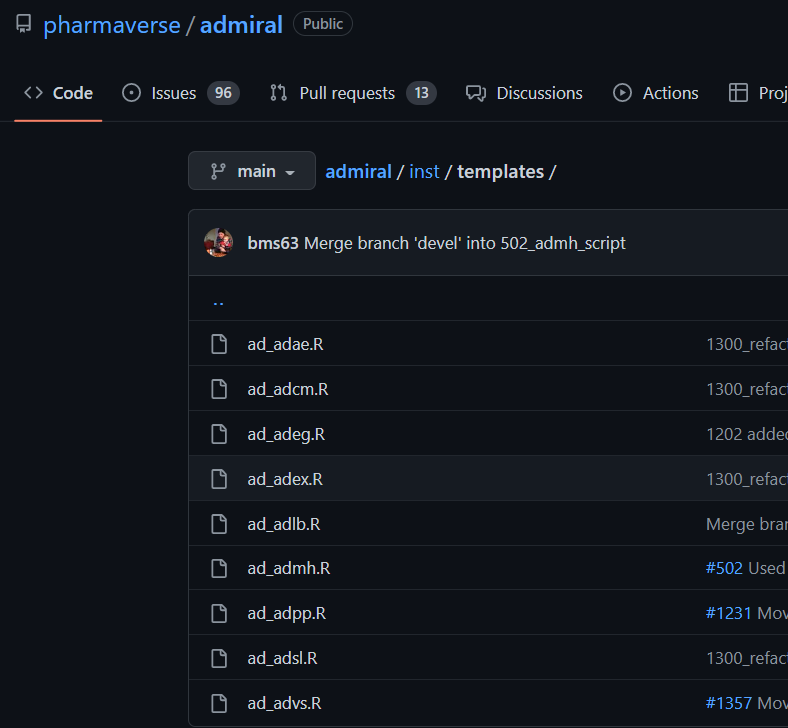
\includegraphics{templates.png}

\hypertarget{cicd-for-templates}{%
\subsection{CI/CD for Templates}\label{cicd-for-templates}}

\begin{itemize}
\tightlist
\item
  After a Code Review the template code is executed
\item
  If any errors or warnings are detected the CI/CD check fails and the
  contributor must fix the error or warning.
\end{itemize}

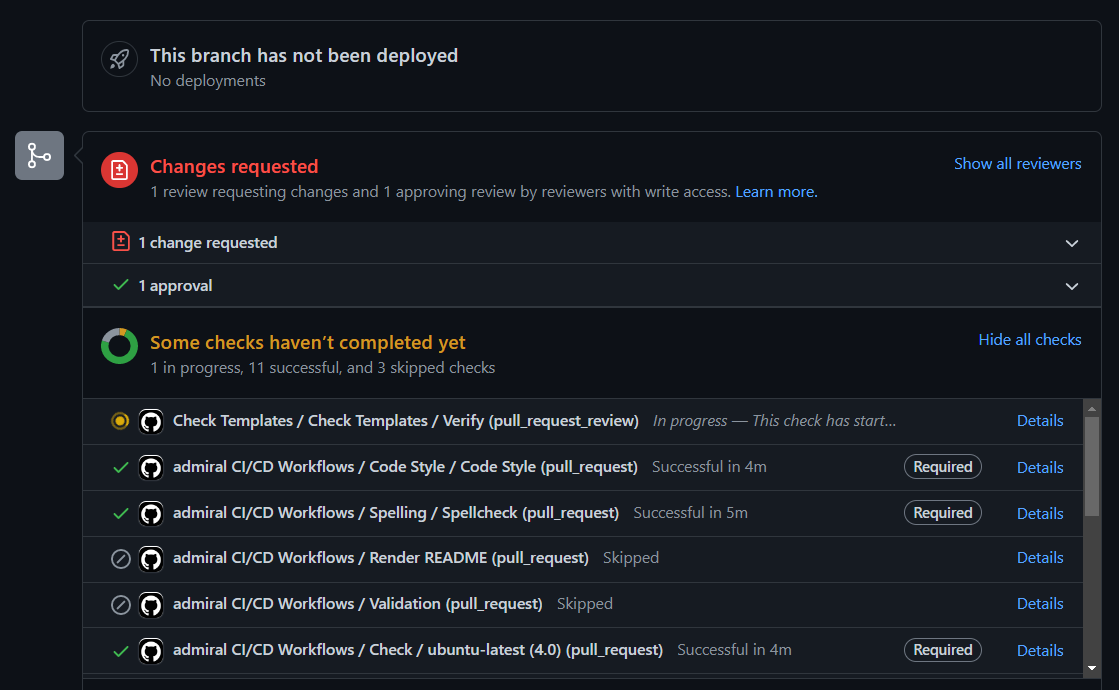
\includegraphics{template_review.png}

\hypertarget{issue-2-admiral-upstream-and-downstream-dependencies}{%
\subsection{Issue 2: admiral upstream and downstream
dependencies}\label{issue-2-admiral-upstream-and-downstream-dependencies}}

\begin{itemize}
\tightlist
\item
  As you can imagine there can be a lot of different types of ADaMs!
\item
  Extension packages focus on specific disease areas like oncology
\item
  The admiral family has a package for developers, template R package
  repo, dummy data
\item
  Eek!! How to keep this all in line!
\end{itemize}

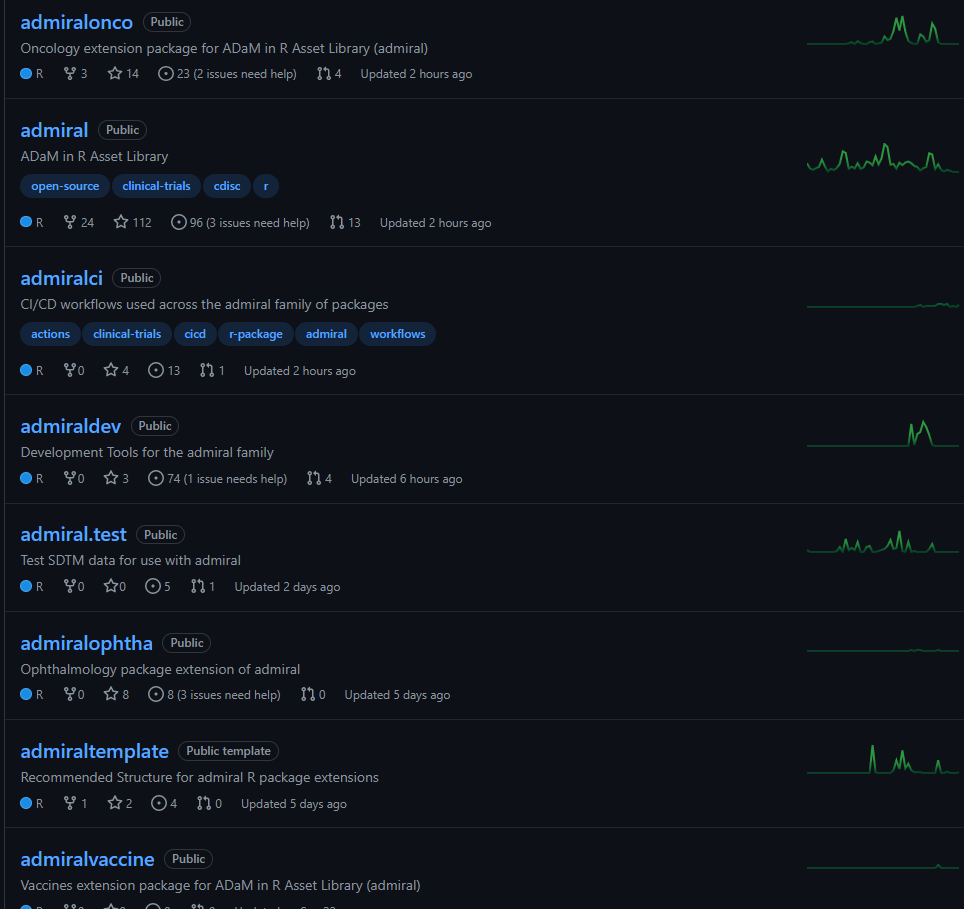
\includegraphics{admiralext.png}

\hypertarget{issue-2-common-cicd-workflows-for-admiral-upstream-and-downstream-dependencies}{%
\subsection{Issue 2: Common CI/CD workflows for admiral upstream and
downstream
dependencies}\label{issue-2-common-cicd-workflows-for-admiral-upstream-and-downstream-dependencies}}

\begin{itemize}
\tightlist
\item
  As you can imagine there can be a lot of different types of ADaMs!
\item
  Extension packages focus on specific disease areas like oncology
\item
  The admiral family has a package for developers, template R package
  repo, dummy data
\item
  Eek!! How to keep this all in line!
\end{itemize}

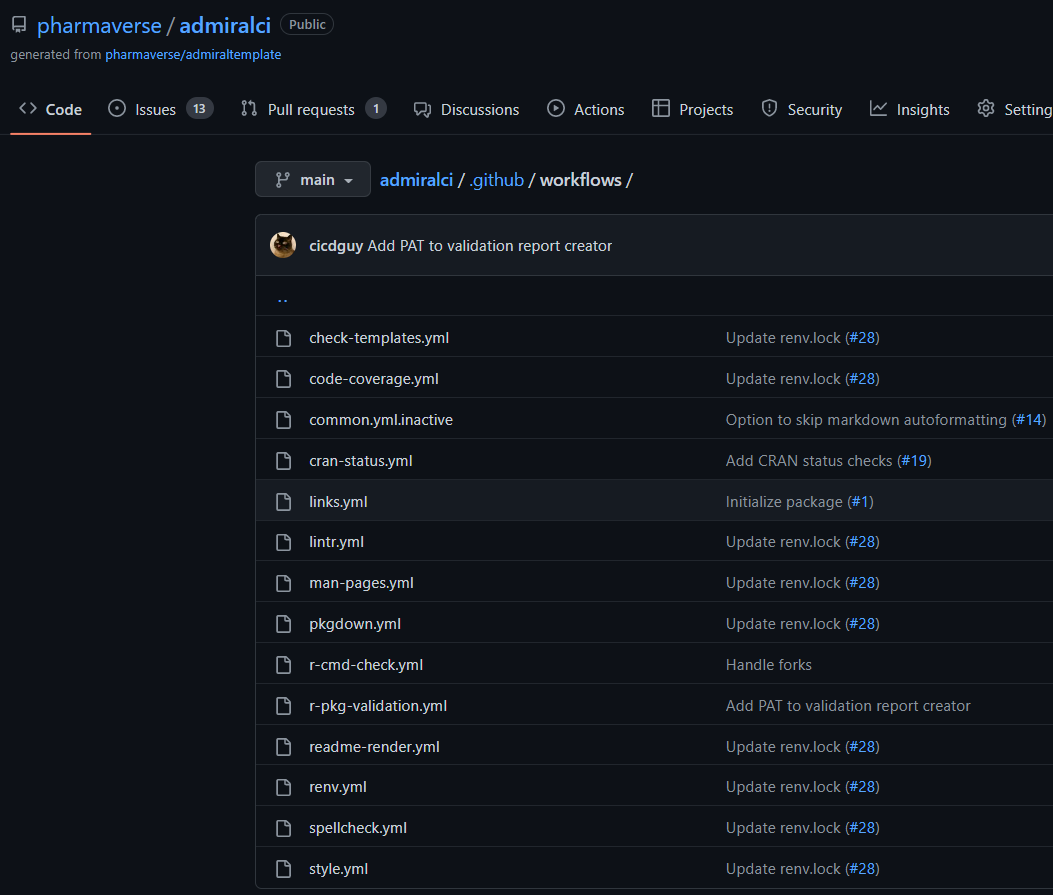
\includegraphics{admiralci.png}

\hypertarget{need-to-give-confidence-that-our-package-is-reliable}{%
\subsection{Need to give confidence that our package is
reliable}\label{need-to-give-confidence-that-our-package-is-reliable}}

CICD ``validation'' job to create a small report that emulates the sort
of validation reports that get made locally

\hypertarget{shiny-app-testing}{%
\subsection{Shiny App Testing}\label{shiny-app-testing}}

How NEST run Shiny apps tests

\hypertarget{case-study---rbmi}{%
\section{Case Study - rbmi}\label{case-study---rbmi}}

\hypertarget{about-rbmi}{%
\subsection{About RBMI}\label{about-rbmi}}

\begin{itemize}
\tightlist
\item
  Reference Based Multiple Imputation
\item
  Implements imputation for longitudinal data in accordance with the ICH
  E9(R1) Addendum on Estimands
\item
  Acknowledgements to Alessandro Noci, Marcel Wolbers \& Daniel Sabanes
  Bove
\item
  Links

  \begin{itemize}
  \tightlist
  \item
    \url{https://arxiv.org/abs/2109.11162}
  \item
    \url{https://github.com/insightsengineering/rbmi}
  \end{itemize}
\end{itemize}

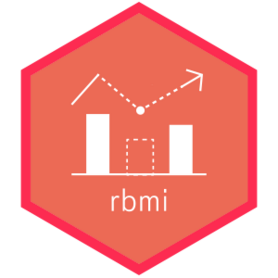
\includegraphics{rbmi.png}

Key component of the package is that many of the methods rely on
resampling techniques to generate confidence intervals. This requires
fitting potentially 1000's of MMRM models which means run times tend to
be in the order of minutes to hours for a full run of the package
depending on the size of the data

\hypertarget{package-development-problems}{%
\subsection{Package Development
Problems}\label{package-development-problems}}

\begin{itemize}
\tightlist
\item
  Installation takes \textgreater3 minutes to compile STAN code
\item
  Full test suite takes \textgreater50 minutes to run
\item
  Vignettes took \textgreater5 minutes to run
\item
  Need to release on in-house servers running legacy versions of R
\item
  Many PR's forgot to run \texttt{devtools::document()}
\item
  Many PR's forgot to rebuild pkgdown site
\end{itemize}


\includegraphics{sad-emoji.png}

2 key issues that we are about to cover: - Need to get run times down to
\textless10 minutes - Need to ensure package works both on internal
server and CRAN

\hypertarget{reducing-the-test-suite-runtime}{%
\subsection{Reducing the Test Suite
Runtime}\label{reducing-the-test-suite-runtime}}

\begin{Shaded}
\begin{Highlighting}[]
\FunctionTok{test\_that}\NormalTok{(}\StringTok{"Some long running section"}\NormalTok{, \{}
  
    \FunctionTok{skip\_if\_not}\NormalTok{(}\FunctionTok{Sys.getenv}\NormalTok{(}\StringTok{"R\_TEST\_FULL"}\NormalTok{) }\SpecialCharTok{==} \StringTok{"TRUE"}\NormalTok{)}
    
    \CommentTok{\# \textless{}rest of the test code\textgreater{}}
    
\NormalTok{\})}
\end{Highlighting}
\end{Shaded}

\begin{Shaded}
\begin{Highlighting}[]
\ExtensionTok{on:}
  \ExtensionTok{schedule:}
    \ExtensionTok{{-}}\NormalTok{ cron: }\StringTok{\textquotesingle{}0 4 1,15 * *\textquotesingle{}}
\end{Highlighting}
\end{Shaded}

\hypertarget{need-to-ensure-code-works-on-internal-servers}{%
\subsection{Need to ensure code works on internal
servers}\label{need-to-ensure-code-works-on-internal-servers}}

DockerFile that emulates internal servers + cicd job to ensure code
works in it

\hypertarget{cran-limits-runs-to-10-minutes}{%
\subsection{CRAN limits runs to 10
minutes}\label{cran-limits-runs-to-10-minutes}}

\begin{itemize}
\tightlist
\item
  Extract vignettes to ``as-is'' instead of being built on the fly
\item
  CICD test to then re-build vignettes to make sure they don't error
  (rather than being done in the CRAN-check)
\item
  Extraction of long running unit tests into their own ``extended'' set
  of tests
\item
  CRON CICD job that will run the extended unit tests (which last an
  hour) whilst regular set of unit tests run fine in a couple of minutes
\end{itemize}

\hypertarget{unit-tests-take-a-long-while-to-run-due-to-the-need-to-compile-code}{%
\subsection{Unit tests take a long while to run due to the need to
compile
code}\label{unit-tests-take-a-long-while-to-run-due-to-the-need-to-compile-code}}

Cache the src/ directory so that it is restored on each run (cache done
separately per OS / R-version

\hypertarget{testing}{%
\subsection{Testing}\label{testing}}

\hypertarget{unit-tests}{%
\subsubsection{Unit Tests}\label{unit-tests}}

\begin{enumerate}
\def\labelenumi{\arabic{enumi}.}
\tightlist
\item
  Unit Tests:
\item
  Test Coverage:
\item
  Integration tests:
\end{enumerate}

\hypertarget{static-code-analysis}{%
\subsection{Static Code Analysis}\label{static-code-analysis}}

\begin{enumerate}
\def\labelenumi{\arabic{enumi}.}
\tightlist
\item
  Linting
\item
  Spell Check
\item
  Link \& URL Checks
\end{enumerate}

\hypertarget{documentation}{%
\subsection{Documentation}\label{documentation}}

\begin{enumerate}
\def\labelenumi{\arabic{enumi}.}
\tightlist
\item
  Man pages
\item
  pkgdown site
\end{enumerate}



\end{document}
